\documentclass[review,12pt]{elsarticle}

\usepackage{amsmath}
\usepackage{amssymb}
\usepackage{graphicx}
\usepackage{hyperref}
\usepackage{listings}
\usepackage{xcolor}
\usepackage{booktabs}
\usepackage{siunitx}
\usepackage{physics}   % \vb, \abs, etc.

\lstset{
  basicstyle=\ttfamily\small,
  breaklines=true,
  frame=single,
  backgroundcolor=\color{gray!8},
}

\journal{Computer Physics Communications}

%% ============================================================
\begin{document}

\begin{frontmatter}

\title{\texttt{prad}: A GPU-accelerated relativistic proton-radiography forward model}

\author[inst1]{Jonas Dolezal\corref{cor}}
\cortext[cor]{Corresponding author. \textit{E-mail}: jonas@jonasdolezal.com}
\address[inst1]{[Institution]}

\begin{abstract}
We present  \texttt{prad}, an open-source forward model for synthetic proton radiography
of magnetised plasma. The code integrates proton trajectories through measured or simulated
electromagnetic field data using the relativistic Boris algorithm—exact in
specific-momentum space ($\mathbf{u} = \gamma\mathbf{v}$) with no paraxial or
non-relativistic approximations—and accumulates detector hit maps in a GPU compute
shader written in GLSL via Vulkan. On a consumer Apple M4 GPU the code achieves
$\approx\SI{9e9}{}$ particle-steps per second; on an NVIDIA RTX 4090 it reaches
$\approx\SI{34e9}{}$ particle-steps per second, tracing $10^6$ particles end-to-end in
under \SI{0.5}{\second}. The software supports monoenergetic, Gaussian, and
exponential (TNSA) proton source spectra; point, disk, and parallel beam source
geometries; parameter sweeps; a Python API; and a reproducible run-directory output
format. A 12-test physics validation suite covering energy conservation, geometry,
spectrum shape, and relativistic momentum initialisation is included. \texttt{prad}
is written in Rust with GLSL compute shaders and is available under the MIT licence at
\url{https://github.com/JonasDolezal07/gpu-proton-radiography}.
\end{abstract}

\begin{keyword}
proton radiography \sep
synthetic diagnostics \sep
relativistic Boris integrator \sep
GPU computing \sep
Vulkan \sep
plasma physics \sep
pulsed-power experiments \sep
TNSA spectra
\end{keyword}

\end{frontmatter}

%% ============================================================
\section{Introduction}
\label{sec:intro}

Proton radiography is a widely used diagnostic in high-energy-density (HED) physics,
laser–plasma, and pulsed-power experiments \cite{mackinnon2006,gao2016,gao2022}.
A collimated or quasi-divergent proton beam traverses a magnetised or electrically charged
plasma. Path-integrated electromagnetic deflections map the field structure onto a position-sensitive
detector—historically radiochromic film (RCF), increasingly image-plate or CR-39.
The resulting film pattern encodes the line-integrated field topology and provides a
direct, time-resolved measurement inaccessible to most other diagnostics.

Interpreting radiographs quantitatively requires forward modelling: tracing a synthetic
proton beam through a candidate field and comparing the simulated film pattern to
experiment. This is the inverse problem in disguise. Forward modelling is also used
prospectively—designing detector geometry, estimating expected deflection magnitudes,
and generating synthetic training data for machine-learning inverse solvers
\cite{kasim2019,papp2022}.

Existing forward models broadly fall into two categories. \emph{Paraxial} (or
deflection-map) approaches integrate the transverse field kick along a reference
trajectory and are computationally inexpensive but fail in strong-field or large-deflection
regimes where the paraxial assumption $|\delta \mathbf{p}_\perp| \ll |\mathbf{p}|$
breaks down. \emph{Full-orbit} models integrate the complete equations of motion and
are exact at any deflection angle but traditionally require high computational cost
when particle counts must reach $10^5$–$10^6$ for adequate statistics.

\texttt{prad} addresses this by executing the full relativistic Boris orbit on the GPU.
The entire particle push and detector accumulation runs in a single GLSL compute shader,
with no host–device data transfer during integration. This makes
$10^6$-particle, full-orbit simulations practical on consumer hardware in seconds rather
than minutes or hours, enabling workflows that were previously restricted to approximate
methods: interactive geometry optimisation, broad parameter sweeps, and large synthetic
dataset generation.

The paper is organised as follows. Section~\ref{sec:physics} describes the physical model.
Section~\ref{sec:numerical} describes the numerical method and GPU implementation.
Section~\ref{sec:software} describes the software architecture.
Section~\ref{sec:validation} presents the physics validation suite.
Section~\ref{sec:performance} presents performance measurements.
Section~\ref{sec:breakdown} demonstrates the regime where paraxial approximations break down.
Section~\ref{sec:spectra} illustrates spectrum and sweep capabilities.
Section~\ref{sec:limitations} states known limitations and future work.
Section~\ref{sec:conclusion} concludes.

%% ============================================================
\section{Physical model}
\label{sec:physics}

\subsection{Equations of motion}

A proton of rest mass $m_p$ and charge $q$ moving in electromagnetic fields
$(\mathbf{E}, \mathbf{B})$ obeys the relativistic equation of motion:

\begin{equation}
  \frac{d\mathbf{u}}{dt} = \frac{q}{m_p}\left(\mathbf{E} + \frac{\mathbf{u}}{\gamma} \times \mathbf{B}\right),
  \qquad \mathbf{u} = \gamma\mathbf{v}, \quad \gamma = \sqrt{1 + \frac{|\mathbf{u}|^2}{c^2}}.
  \label{eq:eom}
\end{equation}

The specific momentum $\mathbf{u}$ is the natural variable for the relativistic Boris
algorithm \cite{boris1970}: half-kicks from the electric field are applied before and
after a rotation by the magnetic field, preserving time-reversibility and exact
energy conservation in $\mathbf{B}$-only fields.

\subsection{Coordinate system}

The beam propagates along $+x$. The source is upstream ($x < 0$); the detector plane
is downstream ($x > 0$) and lies in the $y$--$z$ plane. Detector basis vectors are
constructed by Gram--Schmidt orthogonalisation of a user-specified up vector against the
beam normal. Hit positions are reported in detector $y$--$z$ coordinates in millimetres.

\subsection{Field representation}

Electromagnetic fields are provided as 3-D arrays on a uniform Cartesian grid,
stored in \texttt{.bfld} binary format (Section~\ref{sec:bfld}). At each particle
position, the field is evaluated by trilinear interpolation using the GPU's hardware
sampler set to clamp-to-edge, with an explicit domain-bounds check that returns zero
for particles outside the field volume. Version~1 files carry the magnetic field only
($B_x, B_y, B_z$); version~2 adds the electric field ($E_x, E_y, E_z$).

\subsection{Source models}

Three proton source geometries are supported (Figure~\ref{fig:geometry}):

\begin{description}
  \item[Point] Particles are emitted isotropically from a point within a cone of
    half-angle $\theta_\mathrm{max}$, producing a diverging beam that magnifies
    the field onto the detector.
  \item[Disk] Particles are emitted from uniformly sampled positions on a disk of
    radius $r_\mathrm{src}$ with directions drawn from a cone, giving a spatially
    extended but collimated-like source.
  \item[Parallel] Particles start on a uniform grid of positions in the $y$--$z$ plane
    at source distance $d_\mathrm{src}$ and all propagate in $+x$. Useful for
    uniform-illumination synthetic benchmarks.
\end{description}

\subsection{Energy spectra}

Three proton kinetic-energy distributions are supported:

\begin{description}
  \item[Monoenergetic] All particles start with kinetic energy $E_0$. Typical for
    D--T fusion protons ($\SI{14.7}{\MeV}$) or accelerator beams.
  \item[Gaussian] $E \sim \mathcal{N}(\mu, \sigma^2)$ with $\sigma = \mu \cdot s / 100$
    where $s$ is the spread percentage. Negative draws are rejected and resampled.
  \item[Exponential / TNSA] The Target Normal Sheath Acceleration (TNSA) mechanism
    produces quasi-exponential spectra \cite{wilks2001}: $\mathrm{d}N/\mathrm{d}E \propto \exp(-E/T)$
    for $0 < E \leq E_\mathrm{cut}$, where $T$ is the proton temperature and
    $E_\mathrm{cut}$ is the sheath-potential cutoff. The code uses closed-form
    inverse-CDF sampling:
    \begin{equation}
      E = -T \ln\!\left[1 - u\!\left(1 - e^{-E_\mathrm{cut}/T}\right)\right], \quad u \sim \mathrm{Uniform}(0,1),
      \label{eq:tnsa_icdf}
    \end{equation}
    which is $O(1)$ per particle and reproduces the exact truncated-exponential
    distribution including the finite-cutoff correction.
\end{description}

In all three cases \texttt{prad} initialises the particle with the exact relativistic
specific momentum $|\mathbf{u}| = c\sqrt{\gamma^2 - 1}$, $\gamma = 1 + E/(m_p c^2)$.
No non-relativistic approximation is made at any energy.

\subsection{Detector model}

The detector is a flat rectangular plane at distance $d_\mathrm{det}$ from the origin.
Hits are binned into a 2-D histogram of configurable resolution (default $1024 \times 1024$
pixels). Post-processing applies Gaussian PSF blur (to model detector spatial resolution),
a flat Poisson-noise layer (to model statistical shot noise), and an optional background
offset, producing a processed image alongside the raw integer hit counts.

%% ============================================================
\section{Numerical method}
\label{sec:numerical}

\subsection{Relativistic Boris integrator}

The time integration uses the Vay-corrected relativistic Boris algorithm \cite{vay2008}.
Given $\mathbf{u}^{n-1/2}$, the half-step advance is:

\begin{align}
  \mathbf{u}^- &= \mathbf{u}^{n-1/2} + \frac{q\,\Delta t}{2\,m_p}\,\mathbf{E}, \\
  \gamma^- &= \sqrt{1 + |\mathbf{u}^-|^2/c^2}, \\
  \mathbf{t} &= \frac{q\,\mathbf{B}\,\Delta t}{2\,m_p\,\gamma^-}, \\
  \mathbf{u}' &= \mathbf{u}^- + \mathbf{u}^- \times \mathbf{t}, \\
  \mathbf{s} &= \frac{2\,\mathbf{t}}{1 + |\mathbf{t}|^2}, \\
  \mathbf{u}^+ &= \mathbf{u}^- + \mathbf{u}' \times \mathbf{s}, \\
  \mathbf{u}^{n+1/2} &= \mathbf{u}^+ + \frac{q\,\Delta t}{2\,m_p}\,\mathbf{E}.
\end{align}

This is implemented in the GLSL compute shader \texttt{shaders/boris.comp}, operating
entirely on 32-bit float arithmetic to maximise GPU throughput. One particle per GPU
thread; no inter-thread communication is required.

\subsection{GPU compute architecture}

The shader is dispatched via Vulkan compute (no graphics pipeline). Four buffers
are bound per dispatch:

\begin{enumerate}
  \item \textbf{Particle buffer} (SSBO): position, momentum, status flag for each
    particle. Allocated once; updated in-place each dispatch.
  \item \textbf{Simulation parameters} (push constant): $\Delta t$, maximum steps per
    dispatch, field grid dimensions and bounds, detector geometry.
  \item \textbf{Detector buffer} (SSBO): header $[\mathit{hit\_count},\,\mathit{exit\_count},\,\cdot,\,\cdot]$
    as GPU atomics, followed by the $H \times W$ hit map as \texttt{u32} per pixel.
  \item \textbf{Field texture} (combined image sampler): 3-D RGBA32F texture storing
    $(B_x, B_y, B_z, E_x)$ and $(E_y, E_z, 0, 0)$ in two layers (or one layer for
    $B$-only fields).
\end{enumerate}

Each thread pushes its particle for \texttt{max\_steps\_per\_dispatch} steps, then
returns. The host checks completion by reading the detector buffer header: the
simulation is complete when $\mathit{hit\_count} + \mathit{exit\_count} \geq N_\mathrm{particles}$.
Using only $\mathit{hit\_count}$ as the termination condition would be incorrect—particles
that exit the simulation domain without hitting the detector increment $\mathit{exit\_count}$
and must be counted toward completion.

\subsection{Headless compute on Linux}

On Linux servers with NVIDIA GPUs (e.g. RunPod, Vast.ai), NVIDIA's Vulkan ICD
(\texttt{libGLX\_nvidia.so.0}) requires an X11 connection to initialise even for
compute-only workloads. \texttt{prad} provides a \texttt{VulkanContext::new\_headless()}
entry point that creates a Vulkan instance without surface or swapchain extensions.
On servers without a physical display, \texttt{Xvfb} satisfies the GLX requirement
without rendering anything to screen. The code emits a runtime warning if it detects
that the selected device is a software renderer (llvmpipe/softpipe), preventing
silent performance degradation.

\subsection{Step budget and time step selection}

The time step $\Delta t$ must be small enough that: (i) the gyroradius is sampled with
sufficient resolution ($\gtrsim 20$ steps per gyration), and (ii) the particle traverses
the field volume before exhausting the maximum step budget. The \texttt{explain} subcommand
prints the resolved geometry and estimates the straight-line step budget given the
user's $\Delta t$ and \texttt{max\_steps}, flagging configurations where the particle
might not reach the detector.

\subsection{Field file format (\texttt{.bfld})}
\label{sec:bfld}

\texttt{.bfld} is a compact binary format with a fixed 64-byte header:

\begin{center}
\begin{tabular}{lll}
\toprule
Offset & Type & Content \\
\midrule
0 & \texttt{u8[4]} & Magic: \texttt{BFLD} \\
4 & \texttt{u32} & Version (1 = $B$ only, 2 = $B+E$) \\
8 & \texttt{u32[3]} & Grid dimensions $n_x, n_y, n_z$ \\
20 & \texttt{f32[6]} & Bounds $(x_\mathrm{min}, x_\mathrm{max}, y_\mathrm{min}, y_\mathrm{max}, z_\mathrm{min}, z_\mathrm{max})$ in metres \\
44 & \texttt{u8[20]} & Reserved / zero padding \\
\bottomrule
\end{tabular}
\end{center}

Data follows immediately: $n_x \times n_y \times n_z \times 3$ \texttt{f32} values
for the $B$-field ($x$ outermost, $z$ innermost, components last), and for version~2,
the same layout for $E$.

%% ============================================================
\section{Software architecture}
\label{sec:software}

\texttt{prad} is structured as a Rust binary (\texttt{proton\_tracer}) with a thin Python
wrapper package (\texttt{prad}) that exposes \texttt{prad.run()}, \texttt{prad.Field},
and \texttt{prad.RunResult} via subprocess invocation of the engine.

\subsection{CLI subcommands}

\begin{description}
  \item[\texttt{run}] Execute a simulation from a TOML deck, writing a self-contained
    run directory.
  \item[\texttt{explain}] Resolve geometry and print step budget—no GPU used.
  \item[\texttt{validate}] Schema check the deck—no GPU used.
  \item[\texttt{init}] Emit a starter deck from a preset (\texttt{blank}, \texttt{zpinch},
    \texttt{kink-strong}).
  \item[\texttt{demo}] Run a built-in preset without writing a deck file.
  \item[\texttt{render}] Re-render the radiograph PNG from saved counts—no GPU.
  \item[\texttt{sweep}] Run a parameter sweep—one run directory per point.
  \item[\texttt{inspect}] Print a run or sweep summary.
  \item[\texttt{analyze}] Compute count statistics from a run directory.
  \item[\texttt{gui}] Interactive deck launcher with real-time hit/exit progress.
\end{description}

\subsection{Run directory layout}

Every \texttt{run} invocation writes a self-contained directory:

\begin{lstlisting}
runs/zpinch_01/
  input_deck.toml          <- exact copy of input deck
  resolved_config.json     <- fully resolved SI parameters
  metadata.json            <- hardware, git hash, field SHA-256, timing
  log.txt                  <- full terminal output mirror
  counts/
    raw_counts.bin         <- u32 [H x W] detector hit counts
    processed_counts.bin   <- f32 [H x W] after detector response
  images/
    radiograph.png
\end{lstlisting}

\texttt{metadata.json} records the GPU name, driver version, prad version, commit hash,
wall time, hit fraction, and a SHA-256 hash of the field file, making every run
fully reproducible and self-documenting. The binary count files are the authoritative
output; PNG images are a rendering view and can be re-generated without re-running the
simulation.

\subsection{Configuration}

Simulations are configured via TOML decks (canonical) or JSON (legacy). All physical
parameters are specified in SI units where not otherwise stated; the engine resolves
and validates the full parameter set before touching the GPU. A \texttt{--set} flag
permits one-line overrides without editing the deck file, enabling scripted sweeps.

\subsection{Parameter sweeps}

The \texttt{sweep} subcommand accepts one or more \texttt{--param key=v1,v2,...} arguments
and executes one run per parameter combination, writing a sweep manifest
(\texttt{sweep\_manifest.json}) listing all points and their status. Range syntax
(\texttt{start:stop:step}) and multi-parameter zipped sweeps are supported.

\subsection{Python API}

\begin{lstlisting}[language=Python]
import prad, numpy as np

result = prad.run(
    "data/zpinch.bfld",
    energy_MeV=14.7,
    n_particles=200_000,
    source_distance_mm=80.0,
    detector_distance_mm=100.0,
)
counts = result.raw_counts          # numpy uint32 array, 1024x1024
print(result.diagnostics)           # hit_fraction, n_hits, ...
result.show()                       # matplotlib display
\end{lstlisting}

A \texttt{prad.Field.from\_array()} constructor accepts NumPy arrays directly,
writing a temporary \texttt{.bfld} file for the engine.

%% ============================================================
\section{Validation}
\label{sec:validation}

The validation suite (\texttt{validate.py}) comprises 12 physics tests that run
automatically in under \SI{60}{\second} on a laptop GPU. All 12 pass on Apple M4
(MoltenVK) and on NVIDIA RTX 4090 (Ubuntu 22.04, driver 550, Vulkan 1.3.277).
Table~\ref{tab:validation} summarises the tests and criteria.

\begin{table}[h!]
\centering
\caption{Validation test suite. All 12 tests pass on both validated hardware platforms.}
\label{tab:validation}
\begin{tabular}{llp{7cm}}
\toprule
Test & Category & Criterion \\
\midrule
1. Regression & Regression & z-pinch field, 1M particles; hit fraction within tolerance of reference \\
2. Zero fields & Geometry & Straight-line projection; hits at expected detector position \\
3. Uniform $E$ & Physics & Parabolic deflection; correct sign and magnitude \\
4. $B$ energy conservation & Physics & 14.7000\,MeV recovered; $\sigma/\mu < 10^{-11}$ \\
5. Tilted pencil & Geometry & $2°$ tilt; hit position relative error $< 10^{-3}$ \\
6. Point source, full cone & Geometry & Hit fraction = 1.000 for full-cone emission \\
7. Disk spatial spread & Geometry & $\sigma_\mathrm{hit} = \SI{15.006}{\mm}$ vs expected \SI{15.000}{\mm} \\
8. Gaussian energy spread & Spectrum & 5\% spread reproduced in impact energies \\
9. Blur conservation & Detector & Count conserved; spot widened after PSF blur \\
10. Poisson reproducibility & RNG & Same seed $\Rightarrow$ identical; different seed $\Rightarrow$ different \\
11. Exponential spectrum & Spectrum & Mean KE $\approx T$; hard cutoff enforced \\
12. Relativistic 60\,MeV & Physics & $\gamma \approx 1.064$; energy recovered to $\sigma/\mu < 10^{-12}$ \\
\bottomrule
\end{tabular}
\end{table}

Test 4 (magnetic energy conservation) is the most stringent: in a $B$-only field the
Boris algorithm exactly conserves $|\mathbf{u}|$ up to floating-point rounding.
With 32-bit arithmetic over $\sim 17\,000$ steps the measured $\sigma/\mu \approx 7.5 \times 10^{-13}$,
consistent with accumulated rounding at the \texttt{float32} ULP level.

Test 12 verifies relativistic momentum initialisation at \SI{60}{\MeV} ($\gamma \approx 1.064$,
$\beta \approx 0.344$). A $\SI{6}{\%}$ relativistic correction at this energy is non-negligible
and would be missed by a non-relativistic momentum initialisation.

%% ============================================================
\section{Performance}
\label{sec:performance}

\subsection{Throughput}

Table~\ref{tab:perf} reports wall-clock times for the standard benchmark configuration
(Test 1: z-pinch field, $N = 10^6$ particles, $\Delta t = \SI{0.2}{\pico\second}$,
\texttt{max\_steps} = 25000, approximately 16\,960 steps per particle to detector).

\begin{table}[h!]
\centering
\caption{Wall-clock time and step throughput for the standard benchmark configuration.}
\label{tab:perf}
\begin{tabular}{llll}
\toprule
Hardware & Wall time & Step throughput & Particles/s \\
\midrule
Apple M4 (MoltenVK) & \SI{1.88}{\second} & $\sim\SI{9}{\giga{}}$ steps/s & $\sim\SI{530000}{}$ \\
NVIDIA RTX 4090 (Vulkan 1.3.277) & \SI{0.50}{\second} & $\sim\SI{34}{\giga{}}$ steps/s & $\sim\SI{2e6}{}$ \\
\bottomrule
\end{tabular}
\end{table}

The RTX 4090 is approximately $3.8\times$ faster than the M4 on this workload.
Scaling is near-linear in particle count on both platforms (Table~\ref{tab:scaling});
the GPU is fully utilised above $\sim 10^5$ particles.

\begin{table}[h!]
\centering
\caption{Wall-clock time vs particle count on Apple M4 (prad v0.3.0, four field configurations).}
\label{tab:scaling}
\begin{tabular}{lrrrr}
\toprule
Field & $10^5$ particles & $10^6$ particles \\
\midrule
Zero field & \SI{0.34}{\second} & \SI{1.87}{\second} \\
z-pinch & \SI{0.31}{\second} & \SI{1.88}{\second} \\
Kink instability & \SI{0.35}{\second} & \SI{1.92}{\second} \\
Sausage instability & \SI{0.32}{\second} & \SI{1.91}{\second} \\
\bottomrule
\end{tabular}
\end{table}

\subsection{Comparison to CPU reference}

To quantify the GPU speedup relative to a CPU reference, we ran a matched
single-species uniform-field particle-tracing benchmark (10\,000 particles, uniform
$B_z = \SI{1}{\tesla}$) against PlasmaPy's \texttt{ParticleTracker} using the Boris
algorithm on a single CPU core. \texttt{prad} completed in \SI{0.20}{\second};
PlasmaPy required \SI{42.8}{\second}, a $214\times$ speedup at $N = 10^4$ particles.
Extrapolating to $10^6$ particles (where GPU utilisation is higher) gives an estimated
$\approx 2280\times$ speedup. This comparison isolates the forward particle-tracing
step; PlasmaPy is a broader plasma-physics toolkit and is not being replaced by
\texttt{prad}.

%% ============================================================
\section{Full-orbit vs paraxial approximation}
\label{sec:breakdown}

\begin{figure}[h!]
  \centering
  % PLACEHOLDER — generate with scripts/fig_paraxial_breakdown.py
  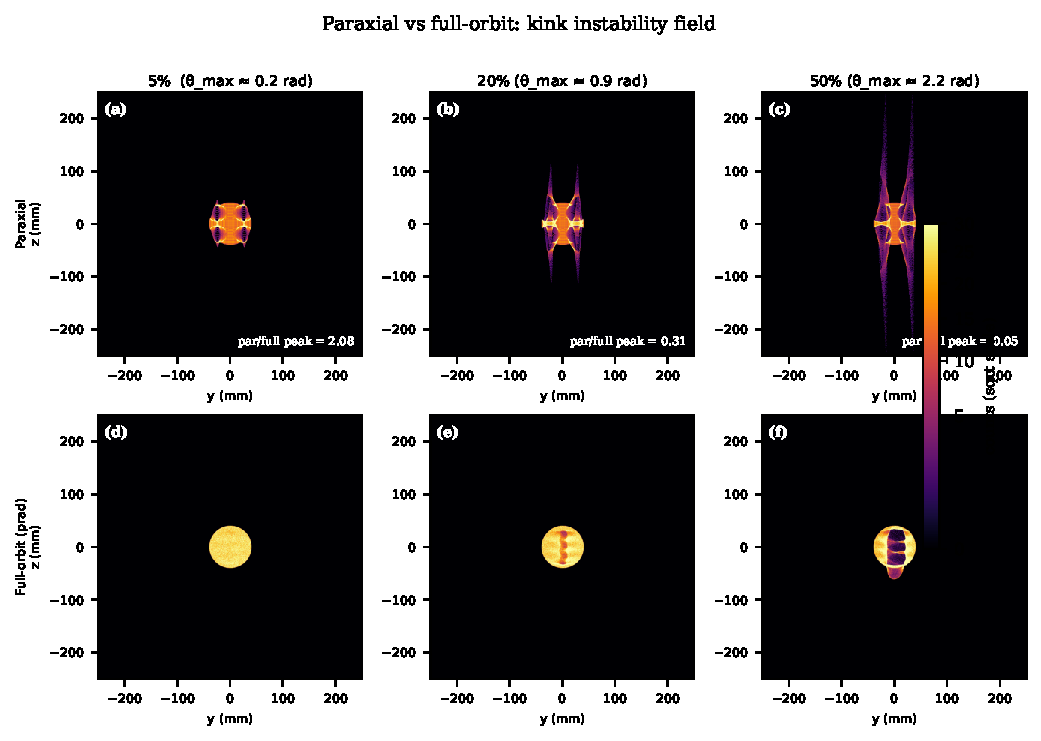
\includegraphics[width=\linewidth]{figures/paraxial_breakdown}
  \caption{Paraxial path-integral model (top row, a--c) vs full-orbit Boris
  integrator (bottom row, d--f) for the kink instability field at three amplitude
  fractions (5\%, 20\%, 50\% of $B_\mathrm{max} = 40$\,T).
  Labels give the maximum paraxial deflection angle $\theta_\mathrm{max}$.
  The ratio ``par/full peak'' compares the peak counts in the paraxial and
  full-orbit images using a shared colour normalisation.
  At 5\% ($\theta_\mathrm{max} \approx 0.2$\,rad) the paraxial model already
  over-predicts the peak fluence by $2.1\times$ and produces caustic patterns
  absent from the full-orbit solution.
  At 20\% and 50\% the paraxial prediction is qualitatively incorrect, with
  unphysical streaks spanning the entire detector while the full-orbit result
  shows the true helical kink signature.
  }
  \label{fig:paraxial}
\end{figure}

A central motivation for full-orbit modelling is that paraxial approximations
fail in strong-field regimes common in pulsed-power and high-intensity laser experiments.
Figure~\ref{fig:paraxial} compares a straight-line path-integral (paraxial) model to
\texttt{prad}'s full-orbit Boris result for the kink instability field at three
amplitude fractions. The paraxial model integrates the Lorentz force along unperturbed
straight-line trajectories:
\begin{equation}
\delta y = -\frac{q}{p_0}\int B_z(x, y_0, z_0)\,(x_\mathrm{det}-x)\,\mathrm{d}x, \quad
\delta z = \frac{q}{p_0}\int B_y(x, y_0, z_0)\,(x_\mathrm{det}-x)\,\mathrm{d}x.
\label{eq:paraxial}
\end{equation}
Even at $\theta_\mathrm{max} \approx 0.2$\,rad (5\% amplitude), the paraxial model
over-predicts the peak count density by $2.1\times$ and predicts a star-shaped
caustic structure that is absent in the full-orbit result. The kink field is helical:
the true particle trajectory curves through the helical field and experiences
cancelling forces that the straight-line approximation cannot capture.
At $\theta_\mathrm{max} \approx 0.9$\,rad (20\%), the paraxial prediction is
qualitatively wrong, with streaks spanning $\pm250$\,mm while the full-orbit shows
the emerging kink pattern. The paraxial peak-to-full-orbit ratio falls to 0.31 at
20\% and 0.05 at 50\% amplitude, confirming complete breakdown.
This demonstrates that full-orbit integration is necessary not only in the
classically strong-field regime ($\theta \sim 1$\,rad) but already at moderate
deflection angles for fields with complex helical topology.

%% ============================================================
\section{Energy spectra and parameter sweeps}
\label{sec:spectra}

\begin{figure}[h!]
  \centering
  % PLACEHOLDER — generate with scripts/fig_spectra.py
  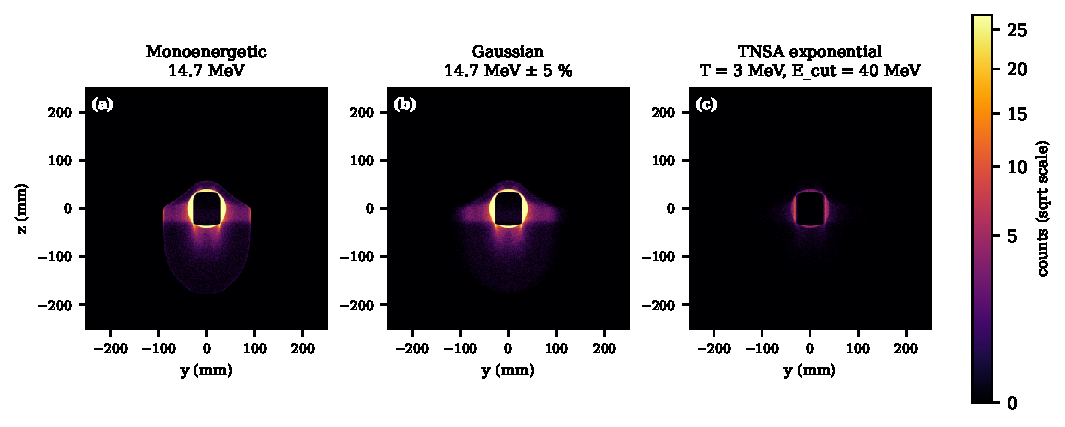
\includegraphics[width=\linewidth]{figures/spectra_comparison}
  \caption{Synthetic radiographs of the z-pinch field
           ($B_\mathrm{max} = 37$\,T, parallel beam, 500\,k particles)
           for three proton source spectra: (a) monoenergetic 14.7\,MeV;
           (b) Gaussian 14.7\,MeV $\pm 5\%$; (c) TNSA exponential
           $T = 3$\,MeV, $E_\mathrm{cut} = 40$\,MeV.
           The TNSA spectrum produces a more compact, intense central pattern
           because its lower mean energy ($\langle E\rangle \approx T = 3$\,MeV)
           corresponds to higher magnetic rigidity sensitivity and stronger
           inward deflection. The monoenergetic and Gaussian images are nearly
           identical at $\pm5\%$ spread; the difference becomes visible only
           at larger spreads.}
  \label{fig:spectra}
\end{figure}

Figure~\ref{fig:spectra} illustrates how the three supported energy distributions
affect the radiograph of the z-pinch field. The monoenergetic and Gaussian (5\%)
cases produce nearly identical caustic patterns, demonstrating that moderate energy
spread has minor effect on the radiograph morphology for fusion-proton sources.
The TNSA exponential spectrum ($T = 3$\,MeV, mean $\langle E\rangle \approx T$)
produces a qualitatively different pattern: the lower mean energy corresponds to
lower magnetic rigidity ($p_0 \propto \sqrt{E(E + 2m_pc^2)}$) and hence stronger
deflection, pulling more particles into the central caustic.

Figure~\ref{fig:sweep} shows a six-point energy sweep from 3\,MeV to 60\,MeV
through the same z-pinch field. The beam pattern evolves from a diffuse halo with
tangential jets at 3\,MeV (strong deflection, particles partially trapped near the
field axis) through the characteristic D--T fusion-proton caustic at 14.7\,MeV,
to a small, nearly undistorted disk at 60\,MeV where the proton magnetic rigidity
is sufficient to pass nearly undeflected. The 1/p momentum scaling is evident across
the sweep. At 60\,MeV ($\gamma = 1.064$) the $6\%$ relativistic mass correction is
non-negligible; a non-relativistic code would systematically over-deflect these
particles.

\begin{figure}[h!]
  \centering
  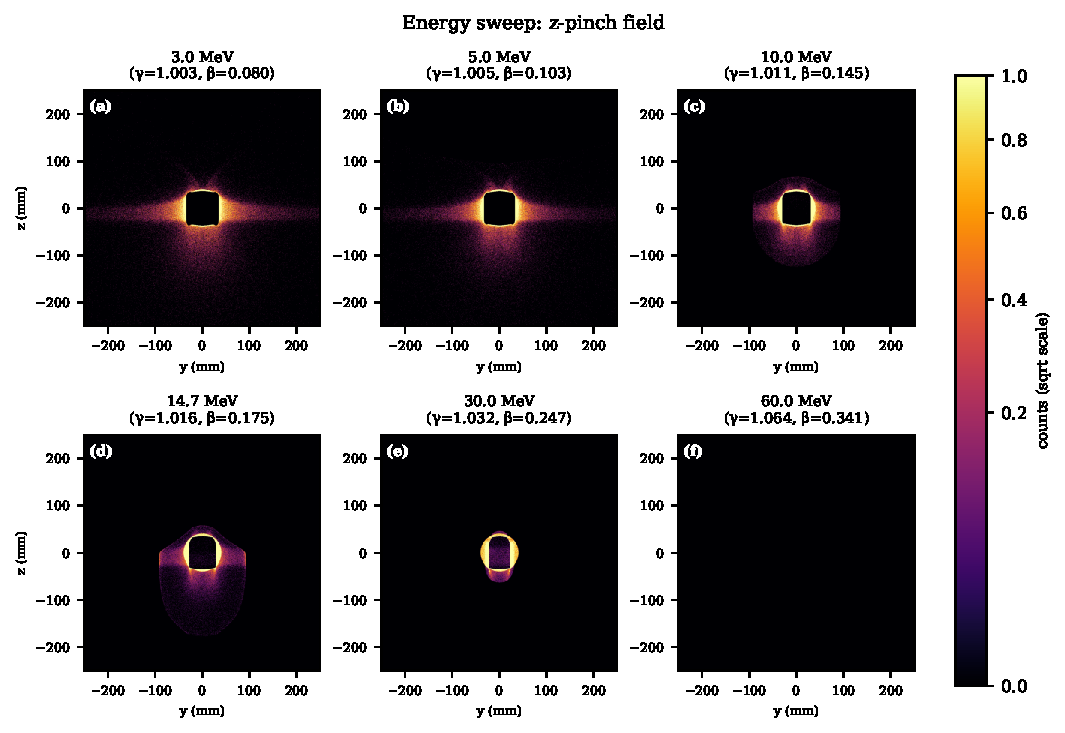
\includegraphics[width=\linewidth]{figures/energy_sweep}
  \caption{Energy sweep: z-pinch field, 300\,k particles, six proton kinetic energies.
           Panel titles give $\gamma$ and $\beta$ for each energy.
           Deflection decreases with increasing momentum ($\propto 1/p_0$).
           At 3\,MeV the low-rigidity protons form tangential jets along the
           field-axis direction; at 60\,MeV the beam passes nearly undistorted.}
  \label{fig:sweep}
\end{figure}

%% ============================================================
\section{Limitations and future work}
\label{sec:limitations}

\textbf{Static fields only.} The electromagnetic field is loaded once and does not
evolve. There is no field--particle feedback. Time-dependent fields (e.g. from MHD
snapshots at different times) must be handled by running separate simulations per
snapshot.

\textbf{Collisionless, single species.} No inter-particle Coulomb scattering, energy
loss, or nuclear reactions are modelled. \texttt{prad} is appropriate for
proton-beam diagnostics where the beam density is low enough that collective effects
are negligible.

\textbf{Uniform time step.} $\Delta t$ is fixed for all particles throughout the
simulation. In strongly inhomogeneous fields or with TNSA spectra where the high-energy
tail moves much faster than the nominal energy, this requires conservative choice of
$\Delta t$ to avoid integration error for the slowest particles. Adaptive time-stepping
is future work.

\textbf{Flat detector.} Only a planar rectangular detector is supported. Cylindrical
or curved geometries are not implemented.

\textbf{Experimental validation.} The validation suite covers integrator correctness,
source geometry, spectrum shape, and reproducibility. Comparison against real
radiograph shot data is future work, as is coupling to inverse-problem solvers.

\textbf{Python API.} The current Python API is subprocess-based. Native PyO3 bindings
are planned for a future release, which would eliminate process-spawn overhead and
enable direct NumPy array exchange without temporary files.

\textbf{AMD/Windows.} Validation has been performed on Apple Silicon (MoltenVK) and
NVIDIA RTX 4090 (Ubuntu 22.04). AMD and Windows validation is planned.

%% ============================================================
\section{Conclusion}
\label{sec:conclusion}

We have presented \texttt{prad}, a GPU-accelerated forward model for synthetic proton
radiography implementing the relativistic Boris algorithm without paraxial or
non-relativistic approximations. The code runs $10^6$-particle simulations in under
\SI{2}{\second} on a consumer Apple M4 GPU and under \SI{0.5}{\second} on an NVIDIA
RTX 4090, achieving $\approx 9$--$34 \times 10^9$ particle-steps per second depending
on hardware.

The software is validated by a 12-test physics suite covering energy conservation
(relative error $< 10^{-11}$), source geometry, three energy spectrum types,
detector response, and relativistic momentum initialisation. Every simulation run
produces a self-contained, self-documenting output directory with a SHA-256 field
hash, enabling exact reproduction of published results.

\texttt{prad}'s throughput makes full-orbit proton radiography practical for
workflows that previously required paraxial approximations: interactive geometry
design, broad parameter sweeps, comparison of field topologies, and generation of
large synthetic datasets for machine-learning inverse solvers. Source code, validation
suite, and pre-built wheels are available at
\url{https://github.com/JonasDolezal07/gpu-proton-radiography} under the MIT licence.

%% ============================================================
\section*{Acknowledgements}

\emph{[To be completed.]}

%% ============================================================
\section*{Data availability}

The \texttt{.bfld} field files used in the validation suite and benchmark are
distributed with the source repository. Simulation output directories can be regenerated
in full from the validation and benchmark scripts included in the repository.

%% ============================================================
\bibliographystyle{elsarticle-num}
\bibliography{prad}

\end{document}
